\begin{flushright} {\tiny {\color{gray} gravity\_exercises.tex}} \end{flushright}
%~~~~~~~~~~~~~~~~~~~~~~~~~~~~~~~~~~~~~~~~~~~~~~~~~~~~~~~~~~~~~~~~~~~~~~~~~~~~~~~~~~~~~~~~~~~~~~~~~~

%The JuPyTer notebook is to be found at:

%\url{https://github.com/ashimrijal/uu_gravity_exercises_2020}


\subsubsection*{Background}

We have seen that the calculation of the gravity vector and/or the gravity potential 
for a mass distribution in 3D space is of the form 
\[
\xi(\vec{r})= {\cal G}  \int_V f(\vec{r},\vec{r}') \rho(\vec{r}') d\vec{r}'
\]
where $\xi$ is either $g_x$, $g_y$, $g_z$ or $U$ and $f$ is a function of the coordinates $\vec{r}$
and $\vec{r}'$.

Let us now assume that the body under consideration can be subdivided into $N_e$ smaller blocks/elements.
By virtue of the linearity of the integral, we have
\[
\xi(\vec{r})={\cal G} \sum_{e=1}^{N_e} \int_{V_e} f(\vec{r},\vec{r}') \rho(\vec{r}') d\vec{r}'
\]
We can further assume that inside each element the density is constant so that 
\[
\xi(\vec{r})={\cal G} \sum_{e=1}^{N_e} \rho_e \int_{V_e} f(\vec{r},\vec{r}') d\vec{r}'
\]
We will now make a strong assumption which is only valid when elements are (very) small:
we will assume that we can replace $f(\vec{r},\vec{r}')$ by $f(\vec{r},\vec{r}_e)$
where $\vec{r}_e$ is the location of the 'center' of the element. We then get:
\[
\xi(\vec{r})= {\cal G}\sum_{e=1}^{N_e} \rho_e  f(\vec{r},\vec{r}_e) \int_{V_e}d\vec{r}'
\]
And finally the integral term is simply the volume of the element $V_e$:
\[
\xi(\vec{r})= {\cal G} \sum_{e=1}^{N_e} \rho_e  f(\vec{r},\vec{r}_e) V_e
\]
In the end, assuming that the body of interest can be split into many small 
elements of constant density, the gravity fields at a location $\vec{r}=(x,y,z)$
can be computed as follows:
\begin{eqnarray}
g_x(x,y,z) &=& {\cal G} \sum_{e=1}^{N_e} \rho_e V_e  \frac{x-x_e}{|\vec{r}-\vec{r}_e|^3} \label{eq:gravdiscr1}\\
g_y(x,y,z) &=& {\cal G} \sum_{e=1}^{N_e} \rho_e V_e  \frac{y-y_e}{|\vec{r}-\vec{r}_e|^3} \label{eq:gravdiscr2}\\
g_z(x,y,z) &=& {\cal G} \sum_{e=1}^{N_e} \rho_e V_e  \frac{z-z_e}{|\vec{r}-\vec{r}_e|^3} \label{eq:gravdiscr3}\\
U(x,y,z)   &=& -{\cal G} \sum_{e=1}^{N_e} \rho_e V_e  \frac{1}{|\vec{r}-\vec{r}_e|}      \label{eq:gravdiscr4}
\end{eqnarray}
where 
\[
|\vec{r}-\vec{r}_e|=\sqrt{ (x-x_e)^2+(y-y_e)^2+(z-z_e)^2   }
\]

The following exercises are designed to test this approach which lends itself to 
numerical implementation. 
The basic idea is rather simple: generate a cloud of points in a regular manner such that 
we can assign them a corresponding volume and a density (and therefore a mass)
when they are in the geometry of interest, 
and then use the formula above to compute the gravity vector and potential, and finally 
compare these values with the analytical solutions we derived for simple spherical bodies. 


{\color{red} All quantities in the code(s) must be expressed in S.I. units, i.e. \si{\metre}, \si{\second}, \si{\kilo\gram}. }

\fbox{NO JUPYTER NOTEBOOK}

%........................................
\subsubsection*{Exercise 1: Full sphere}

\begin{itemize}
\item[(1A)] We consider a domain of size $2R\times 2R \times 2R$ centered on the origin. It is 
partitioned in $N\times N \times N$ cells as shown in the following figure.

\begin{center}
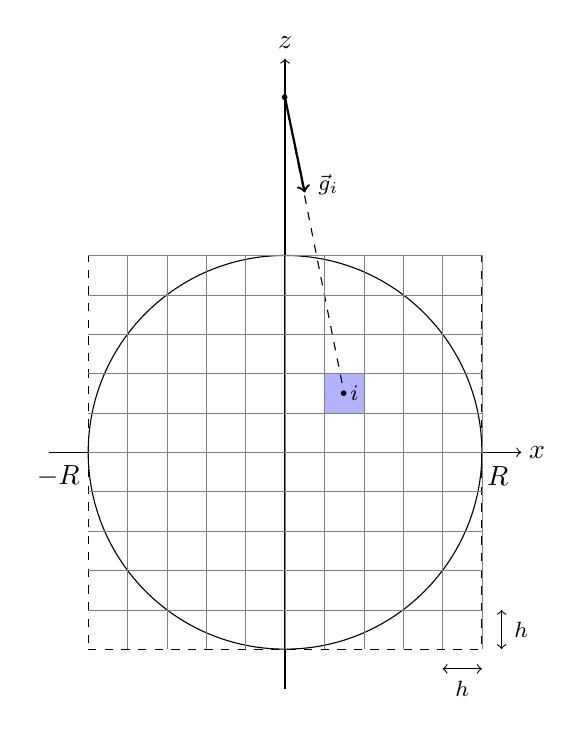
\begin{tikzpicture}
%\draw[fill=gray!23,gray!23](0,0) rectangle (7,9);

%z axis
\draw [->] (3.5,0.5) -- (3.5,8.5);
%x axis
\draw [->] (0.5,3.5) -- (6.5,3.5);

\draw (3.5,3.5) circle (2.5cm);

\draw[dashed] (1,1) -- (6,1) -- (6,6) -- (1,6) -- cycle;

\node[] at (0.62,3.2) {$-R$};
\node[] at (6.2,3.2) {$R$};
\node[] at (6.7,3.5) {$x$};
\node[] at (3.5,8.7) {$z$};

\fill[blue!30!white] (4,4) rectangle (4.5,4.5); %cell i

\draw [dashed] (3.5,8) -- (4.25,4.25);
\draw [->,thick] (3.5,8) -- (3.75,6.8);

\node[] at (4.25,4.25) {\Huge .};
\node[] at (3.5,8) {\Huge .};
\node[] at (4.38,4.25) {\footnotesize $i$};
\node[] at (4.05,6.9) {\footnotesize $\vec{g}_i$};

\draw[<->] (5.5,0.75) -- (6,0.75);
\node[] at (5.75,0.5) {\footnotesize $h$};

\draw[<->] (6.25,1) -- (6.25,1.5);
\node[] at (6.5,1.25) {\footnotesize $h$};

\draw[step=0.5cm,gray,very thin] (1,1) grid (6,6); %grid
\end{tikzpicture}


{\captionfont 2D representation of the exercise. $N=10$}
%\includegraphics[width=3cm]{images/gravity/rubik}
\end{center}

Compute the total number of points {\tt NP} as a function of {\tt N},
the associated volume {\tt dV} of a point (i.e. the volume of the cell the point is in) 
as a function of $R$ and $N$ and  
the size of a cell {\tt h} as a function of $R$ and $N$. Here is 
how your code should look like:
\begin{lstlisting}
N=10
NP=
h=
dV=
\end{lstlisting}

\item[(1B-1)] To get started, start in 1D. Assume that we consider a 1D cube, i.e. the
segment $[-R,R]$ that is divided into $N$ cells. What is $h$?
First, using the {\tt linspace} function compute the $x$-coordinates of the $N$
cell centers. 
Second, compute the same array {\tt x} using a single for loop. 
This second approach will be the building block of the next question.

\item[(1B-2)] 
In the middle of each cell we place a point. Compute and store the coordinates 
of the $N^3$ points (use $R=6371~\si{\kilo\metre}$). Please use 
arrays {\tt x}, {\tt y} and {\tt z} to store the coordinates.
how your code should look like:
\begin{lstlisting}
x = np.zeros(NP,dtype=np.float64) # x coordinates of all points
y = np.zeros(NP,dtype=np.float64) # y coordinates of all points
z = np.zeros(NP,dtype=np.float64) # z coordinates of all points
for i in range(?):
    for j in range(?):
        for k in range(?):
            x[?]=?
            y[?]=?
            z[?]=?
\end{lstlisting}

Important: these arrays are $N^3$ long because they contain the coordinates 
of {\it all} points (cell centers).\\
Help: draw on paper a $3\times3\times3$ elements grid. Place the axis system 
on the plot and explicitely write the arrays for all 27 points. Example:
\begin{verbatim}
x[0]=..... y[0]=..... z[0]=.....
x[1]=..... y[1]=..... z[1]=.....
x[2]=..... y[2]=..... z[2]=.....
...
x[26]=.... y[26]=.... z[26]=.....
\end{verbatim}
Once you have done so, run your code for $N=3$, print the arrays and 
compare their content with what you 
have on paper (tip: for this test temporarily set $R=3$).


\item[(1C)] Assign a density $\rho_0=3000~\si{\kilo\gram\per\cubic\metre}$ to points (cells) 
inside a sphere of radius $R$ and zero otherwise, store these values in the {\tt rho} array.

\begin{center}
\includegraphics[width=5.2cm]{images/geodynamics/rho10}
\includegraphics[width=5.2cm]{images/geodynamics/rho50}
\includegraphics[width=5.2cm]{images/geodynamics/rho150}\\
{\captionfont Example of density field ($\rho=1$) for a $10^3$, $50^3$ and $150^3$ mesh.}
\end{center}


\item[(1D)] Fix $N=10$. Compute the total mass of the sphere
\[
M_s = \int_V \rho \; dV = \sum_{e} \rho_e V_e
\] 
and its volume\footnote{Note that the sums run over the cells which center lies inside the sphere.}
\[
V_s = \int_V \; dV = \sum_{e}  V_e.
\] 

\item[(1E)] Fix $N=10$. Compute the moment of inertia of the sphere 
with respect to rotation axis $z$ using Eq.~\eqref{eq:momI}. 

%In order to compute this quantity we will make use of
%the formula for a spherically symmetric body: 
%\[
%I = \int_V \rho d^2 dV \simeq \sum_i \rho_i d_i^2 dV_i
%\]
%where $d_i$ is the distance of point $i$ to the axis.

\item[(1F)] Repeat the last measurements (1D \& 1E) with different values of $N\in(20,30,40,50,...?)$ .
For both the mass and moment of inertia report on the relative error as a function of $h$.

\item[(1G)] Compute the coordinates of 6 points situated at $z=10^m$ meters 
{\it above the north pole} with $m=0,1,2,3,4,5$ and 
store these coordinates in arrays {\tt xm}, {\tt ym} {\tt zm}. 
\begin{lstlisting}
xm = np.zeros(6,dtype=np.float64) # x coordinates of all points
ym = np.zeros(6,dtype=np.float64) # y coordinates of all points
zm = np.zeros(6,dtype=np.float64) # z coordinates of all points
\end{lstlisting}

\item[(1H)] Fix $N=10$ for now. Compute the gravity potential $U$ and acceleration vector 
components $g_x,g_y,g_z$ at each of these 5 points using Eq.~\eqref{eq:gUexo} (actually its 
discretised version, i.e. Eqs.~\eqref{eq:gravdiscr1}, \eqref{eq:gravdiscr2}, 
\eqref{eq:gravdiscr3} and \eqref{eq:gravdiscr4}.
 
\item[(1I)] Plot the computed quantities as a function of $z$ and plot on 
the same graphic the analytical values. 

\item[(1J)] Fix $m=4$. Progressively increase $N$ and record the absolute error on the gravity vector norm 
as a function of $h$. Plot this in log-log scale. Discuss.

\item[(1K)] Use the {\tt prem\_density} function to assign the PREM \cite{dzan81} density to the points. 
Compute the mass of the planet with this 
new density distribution and compare it with the mass of the Earth. Compute the gravity at the surface.
hint: use a large(r) $N$ for good results. How long are you willing to wait? 

\item[(1L)] Bonus: time how long it takes to compute $U,gx,gy,gz$ at a single location for $N=20$. Report these times. 
Can you think of a way (and implement it) to arrive at the same results in less time?  

\end{itemize}

%..........................................
\subsubsection*{Exercise 2: Hollow sphere}

This is based on the previous exercise. 
\begin{itemize}
\item For points with radius $r$ such that $R/2 \le r \le R$ assign a density $\rho_0=3000\si{\kilo\gram\per\cubic\metre}$ 
and zero otherwise.
\item Compute the gravity potential and vector components on the $x$-axis between $r=0$ and $r=3R$ 
with steps of $R/100$.
\item Plot the results and the analytical solution on the same plot as a function of $r$.
\item Repeat the exercise with different values of $N$. Discuss.
\end{itemize}




%....................................................
\subsubsection*{Exercise 3: Full sphere - revisited}

...NOT for 2024...

We are now going to re-do the first exercise but this time we do not want any point outside of the sphere. 
We shall therefore use the spherical coordinates (see Section~\ref{ss:sphercoord}).
We will use three for loops, one over $r\in[0,R]$ values, 
one over $\theta\in[0,\pi]$ values and one over $\phi\in]-\pi,\pi]$ values. The number 
of points in each direction in this space is still $N$ so that the total number of points is
still $N^3$.

\begin{itemize}
\item Compute and store the coordinates of the points in the $r,\theta,\phi$ space. Store 
these in arrays {\tt r}, {\tt theta}, {\tt phi}.
\item Use these coordinates to compute and store the Cartesian coordinates of these points. 
\item Plot this cloud of points in 3D. Discuss.
\item Repeat the calculations of the first exercise.
\item The cost of the calculation is the same as in exercise 1, but what about accuracy?
\end{itemize}


%....................................................
\subsubsection*{Report}

The report should contain results from exercises 1 and 2. I expect one pdf file per student
(maximum 10 pages) and the corresponding python file(s), all delivered in a single zip file.
Your report does not have to follow questions 1A to 1K in sequential order. 
Please send all files in a single email per {\bf March 29th, 2024, 23:59}. 

You should have the following guidelines in mind when writing your report:
\begin{itemize}
\item Layout: is the document visually pleasing? Is it well structured? are the student names 
and numbers present ?
\item Is there a complete bibliography (if/when applicable)?
\item Introduction: is the context clear? Are the methods presented?
\item Figures: Are they properly numbered? captioned? all figures must be referenced in the text. 
Are they of good quality? are they readable? are all axis labelled?
\item Text: Overall quality of the language. Are there still typos ? Do all sentences make sense?
\item If results are wrong, was an attempt made to document/explain the (probable) source
of the problem?
\item Discussion: are the results properly discussed, analyzed? are potential problems, 
errors, limitations discussed?
\item Conclusion: Are the report's findings summarized and when applicable generalized?
\end{itemize}
For concrete examples of what not to do, check Appendix~\ref{app:grading}.


%what is the resolution one would need to represent the ellipsity of the Earth ?
% compute then moments of inertia
% look at McCullagh formula

%............................................
%\subsubsection{Full sphere - revisited again}
%\url{https://stackoverflow.com/questions/9600801/evenly-distributing-n-points-on-a-sphere/44164075#44164075}
%\begin{lstlisting}
%from numpy import pi, cos, sin, arccos, arange
%import mpl_toolkits.mplot3d
%import matplotlib.pyplot as pp
%num_pts = 1000
%indices = arange(0, num_pts, dtype=float) + 0.5
%phi = arccos(1 - 2*indices/num_pts)
%theta = pi * (1 + 5**0.5) * indices
%x, y, z = cos(theta) * sin(phi), sin(theta) * sin(phi), cos(phi);
%pp.figure().add_subplot(111, projection='3d').scatter(x, y, z);
%pp.show()
%\end{lstlisting}
%\subsubsection{Crust 1.0? s40rts ? }
%measure at random lat lon instead of north pole
